
%(BEGIN_QUESTION)
% Copyright 2006, Tony R. Kuphaldt, released under the Creative Commons Attribution License (v 1.0)
% This means you may do almost anything with this work of mine, so long as you give me proper credit

Some pressure instruments come equipped with {\it chemical seals} consisting of diaphragm units connected to the instrument with small-bore ``capillary'' tubing filled with a liquid such as silicone oil: 

$$\includegraphics[width=15.5cm]{i00216x01.eps}$$

\filbreak

These seals may then be connected to a process vessel to measure pressure, at some distance from the transmitter:

$$\includegraphics[width=15.5cm]{i00216x02.eps}$$

For what purpose(s) do these seals function?  What advantage(s) do they lend to the instrument in measuring pressure?

\underbar{file i00216}
%(END_QUESTION)





%(BEGIN_ANSWER)

Remote, chemical seals provide a means for pressure transmitters to measure the pressure of extremely corrosive process fluids.  The only portions of the instrument in contact with the process fluid are the seal elements themselves: their housings and diaphragms.  The capillary tubing connecting the seals to the transmitter contain only clean oil, as does the transmitter itself.

Now you're probably wondering, ``What's the point of using a remote diaphragm to contact the process fluid?  If the fluid were too corrosive for the transmitter, wouldn't it be too corrosive for the remote seal diaphragm as well?  And if a remote seal can be made to withstand the corrosive effects of the fluid, then why not a regular transmitter?''

For one, pressure transmitters (especially the motion-balance kind) are limited in the kinds materials their pressure elements may be constructed of.  The pressure element (bellows, diaphragm, bourdon tube) must be made of a material with good elastic properties, and that usually means a fairly narrow range of metals.  The seal diaphragms, on the other hand, are designed to be ``slack.''  That is, they are not supposed to provide any spring resistance to motion, but be limp and transfer all the process pressure to the transmitter's sensing element.  Because they need not function as spring elements, their elastic properties are not as critical as for the transmitter's sensing element, and this allows a wider range of materials with different corrosion resistances.  In some cases, the remote diaphragm may be non-metallic, and thus have corrosion resistance properties very different from that of a metal.

Even if the seal diaphragms are metallic, like the transmitter's sensing element, there is still good reason to use chemical seals in some applications.  With a normal pressure transmitter mounted remotely from the process vessel, some kind of tubing will be necessary to transfer fluid pressure to it from the vessel.  The range of available materials for instrument tubing is far more limited than the range of materials for seal diaphragms or even transmitter sensing elements.  It may be that even the best instrument tubing cannot tolerate the corrosive effects of the process fluid, but a seal diaphragm made of some exotic metal alloy can.  Using remote seals and capillary tubes filled with nice, clean oil neatly solves the problem, containing the process fluid within the seals and not allowing it to enter the tubing.

Another, entirely different, reason for using remote seals is in food processing, where no ``pockets'' are allowed in the fluid system due to the need for regular disinfection and decontamination.  Standard $\Delta$P transmitter capsule assemblies and impulse tubing would create cavities for bacteria to collect and grow in nutrient-rich fluid.  Remote seals present a flat surface to the process fluid, transmitting the pressure to the fill fluid where bacteria cannot enter.

A similar reason for using remote seals is to avoid plugging.  With standard ``impulse'' tubes connecting a process vessel or pipe to a transmitter, there exists the possibility of sediment or debris plugging the tubes.  However, flush-mounted remote seals provide no place for sediment or debris to collect.

%(END_ANSWER)





%(BEGIN_NOTES)


%INDEX% Measurement, pressure: chemical seals
%INDEX% Measurement, pressure: remote seals

%(END_NOTES)


